\section{Hardware empleado en el proyecto}
Con el fin de obtener una vista general de todo el proyecto, así como del coste del mismo se lista a continuación todos los componentes del robot y su coste:
\begin{itemize}
	\item Chasis del vehículo. Fabricado a partir de un tablón plano de edf cortado en una cnc láser de forma gratuita gracias al Fablab de la Universidad de Sevilla en la facultad de Arquitectura.
	\item Motores de corriente continua(~1pavos). Adquiridos a través de tiendas digitales destinadas a la importación por un módico precio, lo cual se refleja en una calidad. Sin embargo, formaban parte de un kit que incluye ruedas y acople al eje de transmisión, suponiendo un ahorro importante de tiempo y dinero. 
	\item Encoders ópticos (~6pavos). Compuestos por un diodo emisor de luz ()comprados también en los mismos sitios web que los motores) y por un disco que interrumpe el paso del haz lumínico diseñado específicamente e impreso en 3D.
	\item Microcontrolador ATmega328 (~10pavos). Aunque la gran parte del código implementado en el micro no utiliza las librerías de arduino, por comodidad se ha optado por un microchip ya montado en una placa tipo arduino (un modelo no oficial, clónico).
	\item IMU mpu-6050 (~2pavos).
	\item Raspberry Pi 3B+ (~30pavos). Constituye el cerebro del robot, y centraliza la comunicación con los demás sistemas. Aunque puede resultar el componente más caro del proyecto, se disponían de varias de antemano, por lo que no hubo que asumir su coste.
	\item Kinect for Xbox 360 de Microsoft (~15pavos). Esta popular cámara merece la fama que tiene por lo asequible que es (especialmente el modelo más antiguo) y las utilidades que trae. Se demuestra como la opción más socorrida para desarollar con poco presupuesto aplicaciones que requieran de imágenes o sensores de profundidad.
	
\end{itemize}
\subsection{Estructura}
El robot ha sido diseñado con una topología inspirada en los vehículos de exploración espacial conocidos como \textit{rovers}, utilizando materiales y métodos de construcción asequibles y manteniendo como objetivo una sencilla sustitución e iterabilidad de cada componente. La estructura está diseñada en \textit{FreeCad} y compuesta por piezas de madera mecanizadas en una cortadora láser cnc.
Algunos elementos sin funcionalidad estructural, como los encoders o el soporte de la cámara, han sido fabricados mediante impresión 3D. Todos los modelados pueden encontrarse en la sección hardware de GITHUB.
\begin{figure}[h!]
	\centering
	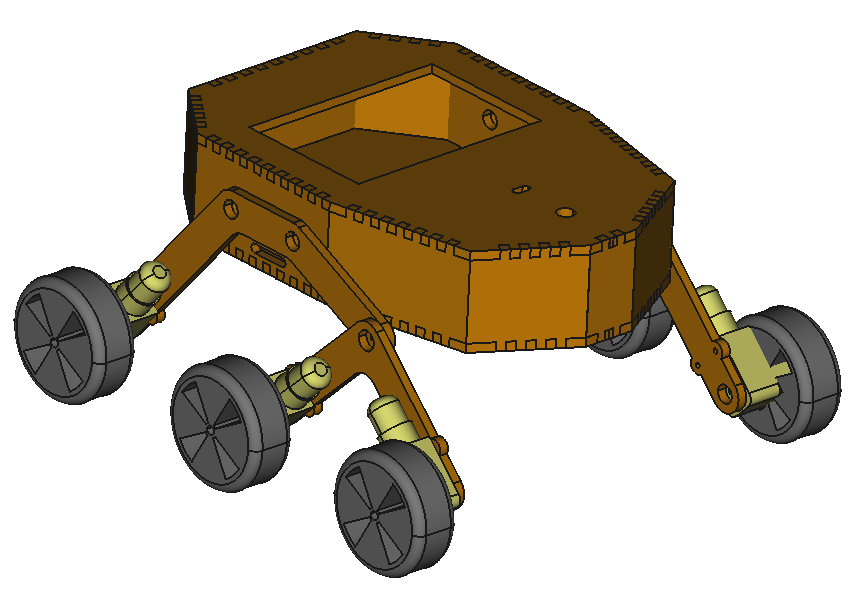
\includegraphics[width=.6\textwidth]{images/wheele_stl}
	\caption{Modelo CAD del robot}
\end{figure}
\\
La disposición geométrica es la de un vehículo diferencial, con tres pares de ruedas, cada una con su respectiva pareja de motor y encoder.\\

\subsection{Motores DC}
 Los seis motores utilizados, a pesar de que deberían comportarse de forma parecida, presentan respuestas muy diferenciadas; para una señal de control idéntica cada uno de ellos muestran puntos de operación distintos y se observan respuestas ante escalón muy variadas. Sin embargo, todos presentan un comportamiento común, una gran zona muerta que complicará mucho la operación del robot a velocidades extremadamente bajas. En concreto, con el convesor digital-analógico del microcontrolador seleccionado (más detalles en la seccion2.arduino), se pierde un 40\% de los bits del rango de salida a causa de este incoveniente.  
 \begin{figure}[h!]
 	\centering
 	
\includegraphics[width=.6\textwidth]{images/hw/motor_est}
 	\caption{Característica estática de un motor}
 \end{figure}
\subsubsection{Especificaciones}
\begin{itemize}
	\item Tensión de trabajo: de (aproximadamente) tres a seis voltios.
	\item Corriente máxima: 120 miliamperios.
	\item Dimesiones: 70x22x18 milímetros.
	\item Reductora: 48 revoluciones a una.
	\item Peso (sin ruedas): 29 gramos.
\end{itemize}
\subsubsection{Drivers}
Debido a las bajas prestaciones y requerimientos de los motores, se ha optado por los drivers más asequibles disponibles: tres microchips L293D que integra cada uno dos puentes H. Como se explica más detenidamente en la seccion SOFEWARE, estos puentes H nos permiten configurar la dirección de giro con dos señales digitales y la velocidad con otras dos señales analógicas.\\
Por comodidad y robustez, se ha diseñado en \textit{KiCad} una placa de circuito impreso muy simple que facilita el cableado y permite integrar algún componente pasivo (como diodos fly-back o capacidades de by-pass). Gracias al laboratorio de electrónica este diseño ha sido revelado sobre una placa de una sola cara, obteniendo, como se aprecia en las imágenes, un acabado final bastante bueno.
 \begin{figure}[h!]
 	\centering
 	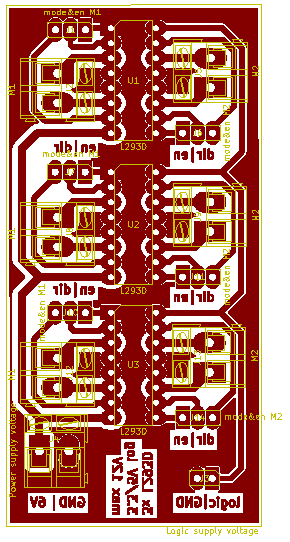
\includegraphics[width=.6\textwidth]{images/hw/pcb_kicad}
 	\caption{Diseño en KiCad de la PCB.}
 \end{figure}
  \begin{figure}[h!]
  	\centering
  	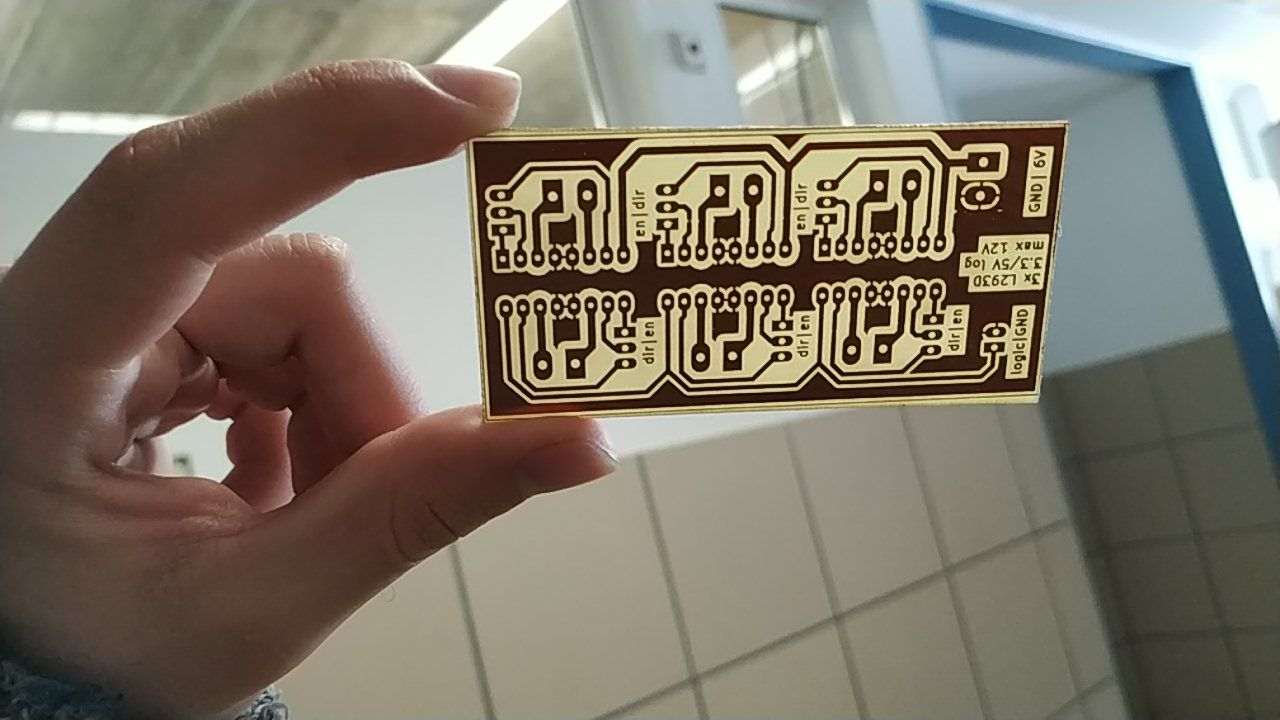
\includegraphics[width=.6\textwidth]{images/hw/pcb_img}
  	\caption{Acabado final de la PCB revelada.}
  \end{figure}
	
\subsection{Encoders}
Los sensores elegidos para medir la velocidad de cada rueda y estimar la posición y velocidad del robot, son unos sencillos encoders ópticos binarios junto a unos discos perforados. Al pasar la luz por una perforación del disco, que gira a la misma velocidad que la rueda, se manda una señal digital al micro. Contabilizando los flancos de subida o de bajada en cierto periódo de tiempo, y conociendo las dimensiones del disco, se obtiene una estimación de la velocidad. Para más detalles en este proceso dirigirese a la ventanilla 3 seccion software encoders GRACIAS. 
 \begin{figure}[h!]
 	\centering
 	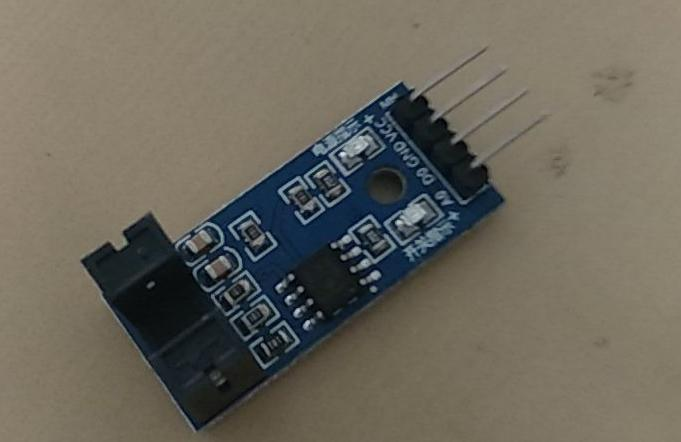
\includegraphics[width=.6\textwidth]{images/hw/encoder_img}
 	\caption{Encoder óptico. En negro resaltan el emisor y recepetor de luz.}
 \end{figure}
  \begin{figure}[h!]
  	\centering
  	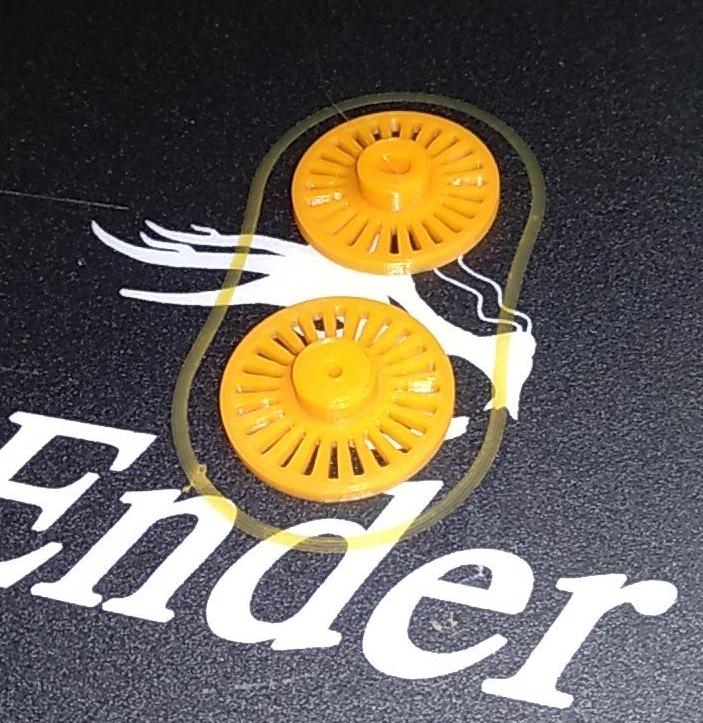
\includegraphics[width=.6\textwidth]{images/hw/encoder_stl}
  	\caption{Disco perforado impreso en 3D.}
  \end{figure}
  
\subsection{IMU}
Como ya se ha mencionado con anterioridad, se ha escogido una IMU mpu-6050 de seis grados de libertad para obtener datos de las velocidades y aceleraciones del robot. El microchip contine varios subsitemas, de los cuales nos interesa resaltar especialmente:
\begin{itemize}
	\item Giroscópio (tres ejes), con un rango progamable de ±250, ±500, ±1000 y ±2000 °/s (grados / segundos).
	\item Acelerómetro (tres ejes), con un rango progamable de ±2g, ±4g, ±8g y ±16g.
	\item Conversores analógico-digitales de 16 bits para las salidas del giroscópio y del acelerómetro.
	\item Bus i2c para ejecutar operaciones de lectura y escritura en cualquier registro del chip a una frecuencia máxima de 400kHz.
	\item Bus de comunicación auxiliar que posibilita introducir un magnetómetro en el futuro sin modificar el conexianado de todo el sistema.
\end{itemize}


\subsection{Controladores de abordo}
\subsubsection{Raspberry Pi}
\subsubsection{Arduino}
\subsection{Cámaras empleadas}
\subsection{Conexionado}